\section{手工特征和强约束先验}
\label{sec:tradition}

\subsection{不同模式水印的攻击方案}

自从水印技术发明以来,研究人员就一直致力于开发去除技术来攻击它们。由于可见水印的多样性,开发鲁棒的可见水印检测和去除方法是一项具有挑战性的任务。更具体地说,可见水印可能由文本、符号、图形等组成,导致从未知和多样化的水印模式中提取有区分性的特征较为困难。此外,不同类型的水印图像中水印的形状、位置、透明度和大小的变化使得在实际情况下难以估计水印嵌入区域。Huang 等~\cite{huang2004attacking}在基于对可见水印及其嵌入特性的基础上,提出了一种只需要少量人工干预的可见水印去除方案。该方案对于完全由细小图案构成的水印,基本的图像恢复(Image Inpainting)技术可以完全去除嵌入的图案。对于更一般的由粗大图案构成的水印,不仅将利用未标记区域的信息,还将利用水印区域内的信息来正确恢复载体图像。尽管所提出的方案不能保证恢复的图像与未标记的原始图像完全相同,但嵌入图案的结构将被严重破坏,并且可以得到一个在感知上令人满意的恢复图像。这一方案的设计,依赖于下述观察:

\begin{itemize}
	\item 由于嵌入的可见水印应该是不显眼的,并且能够保留原始细节,因此水印模式不应包含复杂的纹理或形状结构。事实上,大多数版权模式都是由几种颜色和平坦区域组成的简单的标志或商标。因此,可以合理地假设可行的水印模式是简单的形状和几种固定的颜色,并且普通用户可以轻松选择水印区域的边界。
	\item 嵌入内容中图像细节的可感知性依赖于水印区域内包含的边缘信息的保留。
	\item 用户能够识别水印内容中包含的版权模式主要是因为嵌入模式的形状(轮廓)被保留并且可以与载体内容区分开。如果嵌入的可见水印的轮廓被完全删除或严重扭曲而不引入严重的视觉质量降低,内容所有者将无法再对非法使用者主张其版权。
	\item 可见水印方案的鲁棒性主要在于必须付出大量的人力劳动才能移除水印。因此,一个有效的攻击方案应尽可能少涉及用户干预。但是在攻击过程中,仍然需要某种用户干预,即手动选择水印区域。这是因为目前没有自动识别机制可以正确找出嵌入的水印区域,除非拥有关于水印模式和嵌入参数的特定领域知识。
	\item 为了设计一个通用的攻击机制,只能利用水印内容中的信息。也就是说,在一个带水印的图像中,只有未标记区域中的像素和水印区域内的剩余信息可以在水印去除过程中利用。其他信息,例如嵌入参数或水印图像的实际强度,被假定为未知,因为攻击者只能获取到嵌入的内容。
\end{itemize}

\begin{figure}[!htbp]
	\centering
	\includegraphics[width=\columnwidth]{02.png}
	\caption{可见水印示例}
\end{figure}

对于图案非常简单的可见水印通常由标识受保护数字内容版权的文本、商标或符号组成,并且这些图案的宽度(即线条粗读)通常是有限的。在攻击者选择被嵌入水印图案占据的区域之后,水印攻击问题就类似于图像恢复问题。所选区域可以被视为待恢复的区域,其相应的细节被假设为未知。显然,选定区域与周围未改变区域之间存在很高的相关性;因此,我们可以根据周围未改变区域中包含的强度信息来重新填充这些水印区域。最直接的攻击方法是使用一定大小窗口内所有附近未标记像素的平均强度值来重建水印像素值。水印区域可以逐层缩小,恢复的像素值可用于恢复下一个内部像素。最终,将获得一个近似的水印区域版本。当恢复区域位于原始图像的平坦区域内时,这种平均技术可以获得良好的感知质量,但当水印嵌入在跨越物体边界或包含复杂纹理的位置时,将会出现明显的模糊或伪影,如图 \ref{fig:03}所示。

\begin{figure}[!htbp]
	\centering
	\includegraphics[width=\columnwidth]{03.png}
	\caption{基于平均强度值的恢复结果}
	\label{fig:03}
\end{figure}

图像修复(Image inpainting)技术以不可检测的形式对图像进行修改,以便恢复损坏的区域或移除不需要的对象,其基本思路是来自周围区域的信息被传播到所选区域中。基于修复技术的攻击相比于平均攻击更有效的原因在于前者延长了逼近边缘达到待修复区域边界的过程。整个修复过程可以通过迭代过程实现。

\begin{figure}[!htbp]
	\centering
	\includegraphics[width=\columnwidth]{04.png}
	\caption{基于图像修复的恢复结果}
	\label{fig:04}
\end{figure}

图像修复技术可以成功去除由细线组成的可见水印模式。然而,更常见的水印可能采用由粗线组成的图案。例如,一家公司可能会在其商标或标志中使用粗体或强调的文字来吸引消费者的注意。如果直接在可见水印方案中采用这种类型的模式,水印区域将占据主图像的相当大部分。因此,仅考虑未标记信息的简单图像恢复技术效果不佳。如图\ref{fig:05}所示,显然,与内部水印文字对应的重新填充区域是不正确的。原因很明显:由于正在被攻击的线现在较粗,远离水印区域边界的像素与已知像素的相关性较低,并且仅使用未标记信息无法正确预测它们。在恢复水印区域中心的像素时,来自不同强度的周围区域的信息将相互干扰。

\begin{figure}[!htbp]
	\centering
	\includegraphics[width=\columnwidth]{05.png}
	\caption{粗线水印图案的恢复结果}
	\label{fig:05}
\end{figure}

如前所述,水印在嵌入之后应该保留原始图像的边缘信息。否则,将无法满足图像细节可感知性的要求。一般来说,水印区域和未标记区域可以很容易地分类为边缘区域和平坦区域。此外,由于在攻击开始时用户可以轻松获得水印模式的形状信息,由水印边界分割的平坦区域(即由标记和未标记区域组成的平坦区域)可以被快速识别和提取出来。由于平坦区域内的像素具有相似的强度值,可以根据同一平坦区域内的未标记信息轻松地填充平坦区域内的标记区域。

\begin{figure}[!htbp]
	\centering
	\includegraphics[width=\columnwidth]{06.png}
	\caption{平坦区域恢复原理示意图}
	\label{fig:06}
\end{figure}

如图\ref{fig:07}所示,到目前为止,原始水印图案的形状和结构已经被严重扭曲,大部分重新填充的区域呈现出感知上正确的颜色。尽管某些水印区域保持不变,但嵌入的水印图案已不再可识别。也就是说,嵌入的版权图案现在变得无效。

\begin{figure}[!htbp]
	\centering
	\includegraphics[width=\columnwidth]{07.png}
	\caption{平坦区域恢复结果}
	\label{fig:07}
\end{figure}

尽管可以通过探索剩余的边缘信息来识别和分类所有平坦区域,但只有包含未标记像素的区域才能正确填充。完全位于水印区域内的平坦区域无法获得任何有用的信息,因此只能保持不变。剩下的水印区域现在由完全包含的平坦区域和粗线条水印模式对应区域内的边缘区域组成。

由于使用了水印区域和未标记区域中的所有可用信息,剩余的区域只能通过近似预测来恢复。通过保持边缘和其周围平坦区域之间的强度差异来自动恢复边缘区域,这些区域可能在之前的步骤中原本未被标记或已恢复。边缘的强度根据周围恢复的平坦区域中强度增加或减少的平均量进行调整。尽管水印算法使用的实际颜色变化模型可能非常复杂,并且在攻击过程中不可用,但恢复的边缘区域在感知上是不显眼的。这个结果是合理的,因为边缘区域与周围平坦区域之间的对比仍然保留。虽然无法精确恢复边缘区域的实际强度,但感知的语义得到了很好的保留。实际上,即使在嵌入可见水印之后,由于要求保留原始图像的细节,语义始终存在。

\begin{figure}[!htbp]
	\centering
	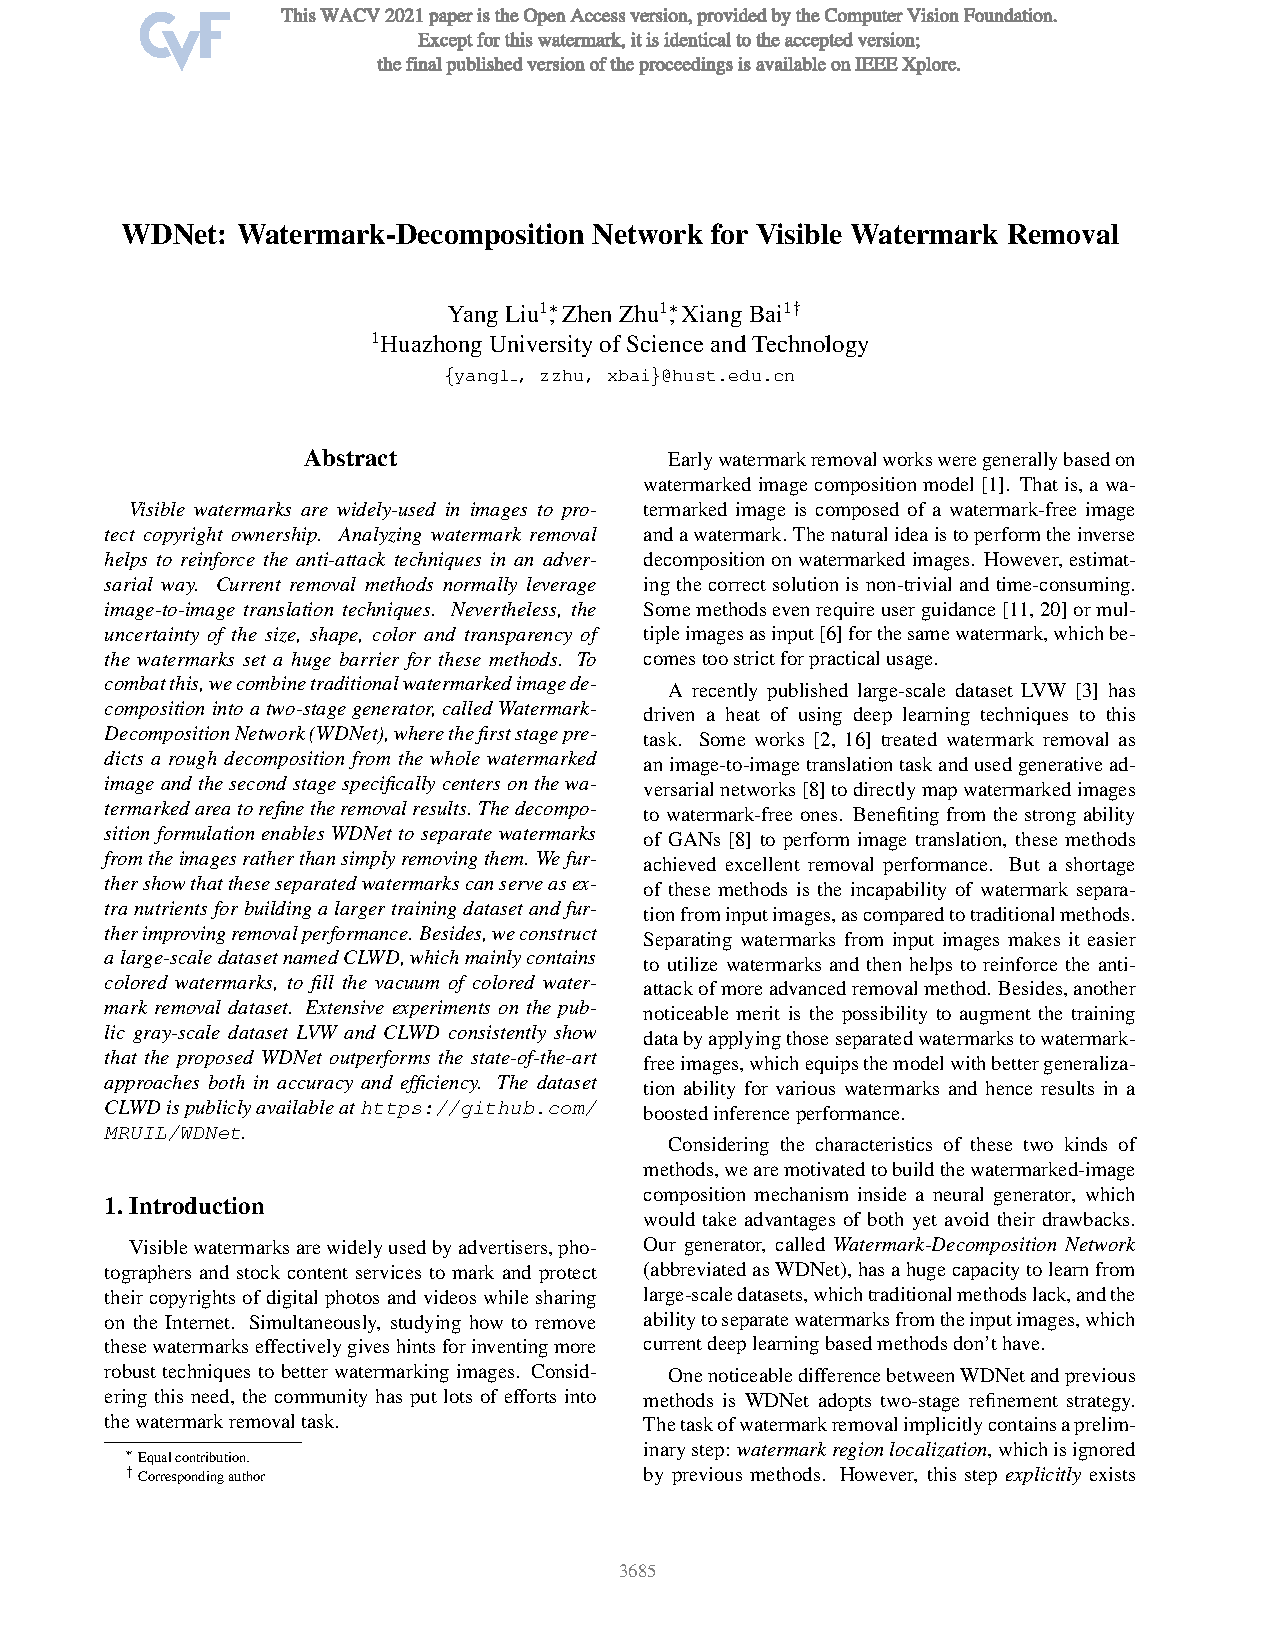
\includegraphics[width=\columnwidth]{08.png}
	\caption{基于可见水印攻击算法的恢复结果}
	\label{fig:08}
\end{figure}

最后,为了恢复完全包含的平坦区域,再次采用了应用于水印边缘区域的相同算法。唯一的区别是根据周围恢复的边缘中出现的像素强度变化量来调整像素强度。由于保留了水印边缘和水印内完全包含的平坦区域之间的差异,恢复的图像在感知上是不显眼的。除了使用预测外,可以统一和手动地调整完全包含的平坦区域的强度值,因为剩余区域非常小且分布稀疏。尽管用户干预是不可避免的,以决定适当的统一强度变化量,但攻击者的工作很简单,因为在提出的攻击的先前阶段已经自动生成了剩余区域的掩码。攻击者可以轻松地迭代地决定适当的强度变化量。

\begin{figure*}[!htbp]
	\centering
	\includegraphics[width=\linewidth]{09.png}
	\caption{基于可见水印攻击算法的恢复结果}
	\label{fig:09}
\end{figure*}

完整的算法流程如下:

\begin{enumerate}
	\item[(i)] 通过用户干预获得表示水印区域的掩码$\mathrm{M}$值;
	\item[(ii)] 应用数学形态学运算操作将$M$分成$\mathrm{M}_{\text {thin }}$和$\mathrm{M}_{\text {thick,}}$两部分,分别表示细线组成的图案和粗线组成的图案相对应的区域;
	\item[(iii)] 通过修复攻击来恢复属于$\mathrm{M}_{\text {thin }}$的区域;
	\item[(iv)] 对整个水印图像的区域使用边缘检测器,并基于阈值  $\mathrm{T}_{\text {edge. }}$将$\mathrm{M}_{\text {thick }}$  分为边缘($\mathrm{M}_{\text {thick }}^{\mathrm{E}}$)和平坦区域($\mathrm{M}_{\text {thick }}^{\mathrm{F}}$);
	\item[(v)] 基于$\mathrm{M}$和$\mathrm{M}_{\text {thick }}^{\mathrm{F}}$,恢复具有未改变近邻的平坦水印区域($\mathrm{M}^{\mathrm{F}-\mathrm{D}}_{thick}$);
	\item[(vi)] Attack remaining edged watermarked areas $\left(\mathrm{M}_{\text {thick }}^{\mathrm{E}}\right)$ by approximated prediction basing on intensity adaptation information of nearby pixels in $\mathrm{M}^{\mathrm{F}-\mathrm{D}}$ thick, obtained in step (v).
	\item[(vii)] 通过基于在步骤(vi)中恢复的$\mathrm{M}_{\text {thick }}^{\mathrm{E}}$的附近像素的强度调整信息的近似预测,攻击完全包含在水印内的平坦区域($\mathrm{m}^{\mathrm{f}-\mathrm{c}}$);	
	\item[(viii)] 如果恢复的图像质量不令人满意,则设置新的阈值$T_{\text {edge }}$,返回步骤(iv),继续迭代。

\end{enumerate}

基于提高可见水印方案鲁棒性的目标,作者提出以下建议:
\begin{enumerate}
	\item[(i)] 在嵌入水印时,应将载体图像的边缘信息视为水印嵌入的参数,因为在平坦区域恢复之后,剩余水印图案的形状极大受到载体图像的边缘结构的影响。例如,将可见水印嵌入到包含高度纹理图案或渐变色分布的区域,无疑会增加水印去除的难度。
	\item[(ii)] 充分增加嵌入图案的形状或纹理复杂性将增加正确选择水印区域的难度。例如,带有抗锯齿边界的水印图案在其精确轮廓之外具有模糊区域。这些模糊区域的强度值与周围透明像素的强度值只有微小的差异,在进行水印选择时可能很容易被忽视。这些区域在经过水印攻击技术后可能介于带水印和未带水印强度值之间,呈现出部分可识别的嵌入图案,需要用户进一步干预。
	\item[(iii)] 为了检测图像是否曾经嵌入可见水印图案,应采用不可见易碎水印(invisible fragile watermarks)技术,即可以使用易碎水印来保护可见嵌入图像的完整性。因此,通过添加不可见易碎水印提供的双重保险,可增强可见水印技术的安全性。当然,在这种情况下,“可见水印方案是否安全?”的问题现在转变为易碎水印的安全问题。
\end{enumerate}

\subsection{强约束的图像组水印去除}

\begin{figure}[!htbp]
	\centering
	\includegraphics[width=\linewidth]{10.png}
	\caption{水印以一致的方式添加到图像集合}
	\label{fig:10}
\end{figure}

可见水印通常包含复杂的结构,如细线和阴影,以增加其难以去除的程度。因此,在没有用户监督或先验信息的情况下,从单张图像中去除水印是一项极其困难的任务。然而,迄今为止,人们忽视了水印以一致的方式添加到许多图像中的事实。例如,内容存储供应商(Stock Content Marketplace)通常在网络上的数百万张图像预览中添加类似版本的水印。基于这一观察,Dekel 等~\cite{dekel2017effectiveness}将图像集合中的水印去除问题形式化为广义的多图像抠图问题,其目标是利用许多观察到的示例来估计“前景”(水印)图像和 $\alpha$ 蒙版,以及“背景”(原始)图像。具体而言,首先利用数据的冗余性提取整个图像集合中一致的图像结构,以获得抠图水印的初始估计,并在所有图像中检测水印区域。然后,通过解决一个优化问题,将抠图水印分离为图像和 $\alpha$ 蒙版组件,同时重建一部分背景图像。

如图\ref{fig:11}所示,第一步是确定图像集合中哪些图像结构属于公共水印,并在所有图像中对它们进行检测。这是一个先有鸡还是先有蛋的问题,因为估计水印需要知道图像中的水印区域,反之亦然。本文通过联合估计抠图水印和在所有图像中检测水印来解决这个问题。具体而言,在以下估计和检测步骤之间进行迭代。

\begin{figure*}[!htbp]
	\centering
	\includegraphics[width=\linewidth]{11.png}
	\caption{自动水印提取流程示意图}
	\label{fig:11}
\end{figure*}


\noindent\textbf{水印估计}:给定当前图像中水印区域的估计,通过观察整个图像集合中一致的图像梯度来确定哪些图像结构属于公共水印。具体而言,在每个像素位置$p$的$x$和$y$方向计算水印图像梯度的中值:

\begin{equation}
\nabla \widehat{W}_m(p)=\operatorname{median}_k\left(\nabla J_k(p)\right)
\end{equation}

当图像数量$K$增加时,不考虑偏移,其将收敛到真实抠图水印$W_m = \alpha W$的梯度。将$I_k$和$J_k$视为随机变量,并计算期望$E [\nabla J_k]$,有:

\begin{equation}
\begin{aligned}
E\left[\nabla J_k\right] & =E\left[\nabla W_m\right]+E\left[\nabla I_k\right]-E\left[\nabla\left(\alpha I_k\right)\right] \\
& =\nabla W_m+E\left[\nabla I_k\right]-\nabla \alpha E\left[I_k\right]-\alpha E\left[\nabla I_k\right] \\
& =\nabla W_m-\nabla \alpha E\left[I_k\right]
\end{aligned}
\end{equation}

其中第二个等式来自于乘法的导数。第三个等式基于自然图像梯度的已知特性, 即在多 图像中具有相同像素位置的强梯度的可能性很小。因此, $\mathrm{E}[\nabla \mathrm{I_k}] \approx 0$ 。这意味着 $\mathrm{E}[\nabla \mathrm{J_k}]$ 近 以于抠图水印 $\mathrm{W_m}$ 的梯度, 除了 $\nabla \alpha \neq 0$ 的像素。在这些像素处, 梯度被 $\nabla \alpha \cdot \mathrm{E}[\mathrm{I_k}]$ 偏移。通过 十算 $\nabla \mathrm{W_m}(\mathrm{p})$ 的幅值并获取其边缘图像的边界框 (使用阈值 0.4 的 Canny 算法) 来裁剪 $\nabla \mathrm{W_m}$ 以去除边界区域。使用泊松重建算法可以获得初始的抠图水印 $\widehat{W}_m \approx W_m$ (经过平移校正)。

\noindent\textbf{水印检测}:给定当前的梯度估计 $\nabla \mathrm{W_m}$, 使用常用于目标检测和识别中的模板匹配的 Chamfer 距离来检测每个图像中的水印。具体而言, 对于给定的水印图像, 使用 Canny 边缘 检测器生成详细的边缘图像, 并计算其欧氏距离变换, 然后将其与 $\nabla \mathrm{W_m}$ (水平和垂直翻转) 进行卷积, 以得到每个像素到最近边缘的 Chamfer 距离。最后, 水印的位置被确定为距离图 中距离最小的像素。这种检测方法非常稳健, 可以在各种不同水印和不同不透明度水平下提供高检测率。

\begin{figure}[!htbp]
	\centering
	\includegraphics[width=\columnwidth]{12.png}
	\caption{初始的水印估计和检测}
	\label{fig:12}
\end{figure}

对于初始化联合估计,如果图像中水印的相对位置是固定的(正如在网络上观察到的任何图像集合的情况),通过将图像相对于它们的中心进行注册并运行步骤I来获得水印梯度$\nabla \mathrm{W_m}$的初始估计。如果水印位置不固定,只需要用户在其中一张图像周围标记一个粗略的边界框。然后,将给定边界框内的梯度作为水印梯度的初始估计。在步骤I和步骤II之间迭代2-3次足以获得准确的检测结果和可靠的抠图水印估计。

在所有输入图像中进行对齐检测后,目标是解决多图像抠图问题,即将每个图像中观测到的亮度分解为其水印、透明度抠图和原始图像组成部分。通过对下列目标进行迭代优化,即可获得嵌入的水印图案和$\alpha$等先验,并进而用于其他图像的水印去除和恢复。

\begin{equation}
\begin{aligned}
& \underset{W, \alpha,\left\{I_k\right\}}{\arg \min } \sum_k\left(E_{\text {data }}\left(W, \alpha, I_k\right)+\lambda_I E_{\mathrm{reg}}\left(\nabla I_k\right)\right) \\
& \quad+\lambda_w E_{\mathrm{reg}}(\nabla W)+\lambda_\alpha E_{\mathrm{reg}}(\nabla \alpha)+\beta E_f(\nabla(\alpha W))
\end{aligned}
\end{equation}

\begin{equation}
E_{\text {data }}\left(I_k, W, \alpha\right)=\sum_p \Psi\left(\left|\alpha W+(1-\alpha) I_k-J_k\right|^2\right)
\end{equation}

\begin{equation}
E_{\mathrm{reg}}(\nabla I)=\sum_p \Psi\left(\left|\alpha_x\right| I_x^2+\left|\alpha_y\right| I_y^2\right)
\end{equation}

\begin{equation}
E_f\left(\nabla W_m\right)=\sum_p \Psi\left(\left\|\nabla W_m-\nabla \widehat{W}_m\right\|^2\right)
\end{equation}

由于此类攻击依赖于图像集合中水印的一致性,一个自然的想法是是否可以通过打破这种一致性来阻止它。因此,本文研究了该攻击对不同类型的不一致性或变化的鲁棒性,这些不一致性或变化有可能在每个图像中嵌入水印时引入。通过实验发现,例如,随机改变水印在整个集合中的位置并不能阻止该攻击检测和去除水印,水印的不透明度或颜色的随机变化也无法阻止。而在嵌入水印过程中对水印进行小的空间变形可以显著降低去除水印后图像的质量,对水印本身几乎没有察觉到的变化。

\begin{figure*}[!htbp]
	\centering
	\includegraphics[width=\linewidth]{13.png}
	\caption{水印去除结果}
	\label{fig:13}
\end{figure*}

\subsection{基于镜头思想的视频水印去除算法}

\begin{figure}[!htbp]
	\centering
	\includegraphics[width=\columnwidth]{14.png}
	\caption{不同视频镜头的两帧}
	\label{fig:14}
\end{figure}

	与多组图像的水印去除不同,视频的水印去除可以依赖于视频的时间连贯性,即在一个帧中被水印遮挡的图像内容在其他帧中是不被遮挡的。通用的视频修复算法为基础的水印去除方法利用下一帧的信息来更好地判断当前图像中缺失的像素值,然而正因为这样的方式不是任意的,因而不能用于在线应用。而且它们具有很高的计算成本,更加抑制了其在真实场景中的应用。为了解决这一问题,Dashti等~\cite{dashti2015video}将视频镜头的思想引入了视频修复算法中。视频镜头是从特定场景中捕捉到的帧序列。如图\ref{fig:14},在足球比赛中,摄像机正在拍摄人群,这是一个视频镜头的一帧,当摄像机改变视角并拍摄裁判员时,这是另一个视频镜头的一帧。每个视频镜头的帧具有结构和统计上的相似性,通常表现出相同类型的纹理。视频镜头是通过计算连续两帧之间的差异的总平均值来定义的。如果这个总平均值足够大,超过了指定的阈值,那么第二帧被检测为新镜头的第一帧。

\begin{figure*}[!htbp]
	\centering
	\includegraphics[width=\linewidth]{16.png}
	\label{fig:fig16}
\end{figure*}

	
在定义了视频镜头的概念后,对视频帧缺失像素的查找和填充只需要集中在相同视频镜头的图像帧即可,从而可以有效减少计算开销。为了填充帧中的水印,在水印周围选择一个面积略大于水印的矩形,然后在当前帧和近邻帧中找到与水印周围矩形中的像素值最匹配的位置。每个矩形框都有一些有效像素和一些无效像素,无效像素位于水印位置上。这样做是希望通过周围有效像素的帮助找到无效像素的最佳值,因此,将紧邻帧中的矩形框向上、向下、向右和向左移动几个像素,以找到与当前帧中的矩形框最佳匹配的位置。最佳匹配与当前帧中矩形框包含的有效像素具有最小均方差(LMSE)。

\begin{figure}[!htbp]
	\centering
	\includegraphics[width=\columnwidth]{15.png}
	\caption{视频水印去除算法样例图}
	\label{fig:15}
\end{figure}

完整的算法流程见上。